\documentclass[submission,copyright]{eptcs}
\providecommand{\event}{UITP 2014} % Name of the event you are submitting to
\usepackage{breakurl}             % Not needed if you use pdflatex only.
\usepackage{amssymb,amsmath}
\usepackage{mathpartir}
\usepackage{verbatim}
\usepackage{saoithin}
\usepackage{tikz}
\usetikzlibrary{arrows,matrix}

%\def\PLAN#1{\textit{\textsf{{#1}}}}
\def\PLAN#1{}
\def\DRAFT#1{}
%\def\DRAFT#1{\textbf{DRAFT: }\textsf{{#1}}}
\def\REVIEW#1{}
%\def\REVIEW#1{\textsc{Review: }\textit{{#1}}}

\title{\UTP2: Higher-Order Equational Reasoning by Pointing}
\author{
  Andrew Butterfield
  \institute{
     School of Computer Science and Statitics\\
     Trinity College Dublin\\
     Ireland}
  \email{Andrew.Butterfield@scss.tcd.ie}
}
\def\titlerunning{UTP2: Reasoning by Pointing}
\def\authorrunning{A. Butterfield}
\begin{document}
\maketitle

\begin{abstract}
We describe a prototype theorem prover, \UTP2, developed to match the style
of hand-written proof work in the Unifying Theories of Programming semantical
framework. This is based on alphabetised predicates in a 2nd-order logic,
with a strong emphasis on equational reasoning.
We present here an overview of the user-interface of this prover,
which was developed from the outset using a point-and-click approach.
We contrast this with the command-line paradigm that continues to dominate
the mainstream theorem provers,
and raises the question: can we have the best of both worlds?
\end{abstract}


\section{Introduction}\label{sec:intro}

Unifying Theories of Programming (UTP) \cite{UTP-book},
is a framework that uses alphabetised predicates to define language
semantics in a relational calculus style, in a way that facilitates
the unification of otherwise disjoint semantic theories,
either by merging them, or using special linking predicates
that form a Galois connection. The framework is designed
to cover the spectrum from abstract specifications
all the way down to near-machine level descriptions,
and as a consequence the notion of refinement plays a key role.

We are doing foundational work in the UTP \cite{UTP-book},
which requires formal reasoning with not only predicates,
but also predicate transformers: $\RR3(P)$ $\defs$ $\Skip \cond{wait} P$
and predicates over predicates: $P = \RR3(P)$.
We also need to use recursion at the predicate level:
$ P \defs \mu Q \bullet F(Q)$,
as well as partially-defined expressions:
$s \le s \cat (tr'-tr) \equiv  tr \le tr'$.
The logic being used is therefore semi-classical
(two-valued logic, but expressions may be undefined)
and of least 2nd-order.
In addition, tool support for foundational work in UTP requires the ability
to easily describe new language constructs,
which can themselves be treated just like predicates,
in keeping with the ``programs are predicates''
philosophy \cite{predprog} of UTP.
In \cite{conf/utp/Butterfield10}
we gave an overview of the Unifying Theories of Programming Theorem Prover
(\UTP2)
that we are developing to support such theory development work%
\footnote{%
In that paper it was called \STHN, but the name has since changed to \UTP2
}%
.
The prover is an interactive tool, with a graphical user-interface,
designed to make it easy to define a UTP theory and to experiment
and perform the key foundational proofs.
The motivation for developing this tool,
rather than using an existing one,
has been discussed in some detail
in \cite{conf/utp/Butterfield10}, but key elements will be reprised here.
The logical and  technical underpinning was further elaborated
upon in \cite{conf/utp/Butterfield12},
which described as being an adapted and generalised version of
the equational reasoning system developed by Tourlakis \cite{journals/logcom/Tourlakis01},
itself inspired by the equational logic of David Gries and his colleagues \cite{gries.93}.

In this paper, we describe how the user interacts
with this theorem prover,
that was developed,
\emph{from the outset},
with the proof and reasoning styles typically used in UTP research and published work.

The key emphasis in development was to use window-based GUI techniques early on as the primary
mode of interaction, in stark contrast to most modern interactive theorem provers
that have essentially a command-line interface (most HOL flavours, CoQ, PVS, \ldots) sometimes wrapped with a
elaborate interface built on top of a highly configurable text editor
(e.g., Proof General on Emacs, new Isabelle/HOL interface on top of jEdit).


\section{Motivation}\label{sec:motivation}

There are a lot of theorem provers in existence,
of which the most prominent feature in \cite{conf/tphol/2006provers}.
Of these, the most obvious candidates for consideration for UTP prover support
are Isabelle/HOL\cite{books/sp/NipkowPW02},
PVS\cite{conf/fmcad/Shankar96},
and CoQ \cite{bk:Coq'Art:04}.
They are powerful, well-supported,
with decades of development experience
and large active user communities.
They all support higher-order logic of some form, with a command-line interface,
typically based around tactics of some form. All three require functions to be total,
but support some kind of mechanism for handling partial functions
(e.g. dependent types in PVS).
Their reasoning frameworks are based on some form of sequent calculus,
and do not support equational reasoning in a native fashion.

There has been work done on improving the user interfaces
of theorem provers of this kind.
An interesting example was ``proof by pointing'' \cite{conf/tacs/BertotKT94}
for CoQ which allowed the user to select a subterm,
whereupon it would generate and apply a tactic based on the subterm's top-level
operator.
Whilst proof-by-pointing is not supported in more recent versions of CoQ,
it has been incorporated into ``Proof General'' \cite{conf/tacas/Aspinall00},
a general purpose user interface for theorem provers, built on top of Emacs.
It supports Isabelle and Coq, among others,
and is basically a proof-script management system.
In essence it supports the command-line tactics of the provers,
allowing the user to edit proof scripts at will,
whilst maintaining prover consistency behind the scenes.
Other explorations in this area include
INKA \cite{Hutter96}, Lovely OMEGA \cite{oai:CiteSeerXPSU:10.1.1.42.1864},
Window inference \cite{Staples95},
Generalized Rewriting in Type Theory \cite{journals/eik/Basin94},
The CoRe Calculus, \cite{conf/cade/Autexier05}
and the Jape Theorem Proving framework (\url{http://japeforall.org.uk/}.)
Of the above, \cite{conf/cade/Autexier05},\cite{journals/eik/Basin94} seems designed
to support equational reasoning, but lack any notion of a GUI. In \cite{Hutter96} and \cite{oai:CiteSeerXPSU:10.1.1.42.1864} we have GUIs, but the logic/proof style is tree based.
The window inference work \cite{Staples95} has a notion of ``focus'' similar to ours,
but has no GUI, and while capable of handling equational rewrites seems to be more general.
Jape has a GUI and facilities to encode logics, but again is deduction-biased, and has no easy 
way to extend the language.





\section{Interaction}\label{sec:interact}

We shall illustrate \UTP2's use by walking through a simple proof,
from a theory of sets, regarding the commutativity of set intersection.

\noindent
We start by launching the theorem prover, and we assume that some theories have been
preloaded: \texttt{Sets}%
\footnote{The \texttt{\$0} suffix is a version number}%
, \texttt{Equality}, \texttt{Logic} and \texttt{\_ROOT} (a base theory always present).
All theories have access to definitions and laws from lower theories.


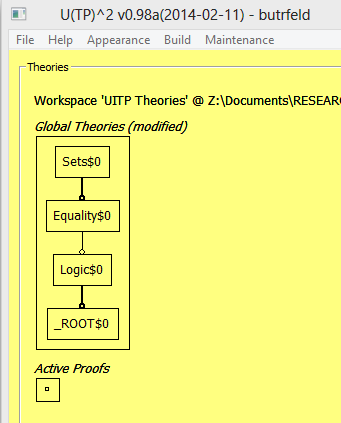
\includegraphics[scale=0.5]{01-initial-state.png}

\noindent
If we double-click on the \texttt{Sets} box,
a window opens up showing the ``Laws'' of the Set theory.
Laws have names, a ``provenance'' indicator, side-conditioning,
and their defining schema (a predicate).

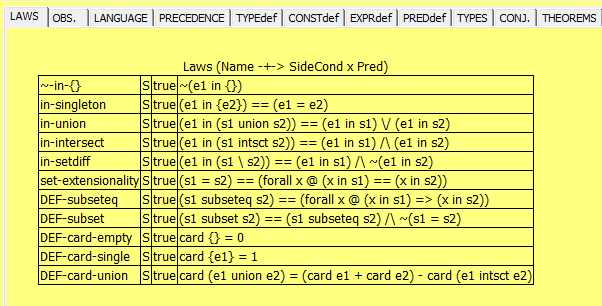
\includegraphics[scale=0.5]{02-set-axioms.png}

\noindent
Clicking on the ``CONJ.'' tab shows some conveniently preloaded conjectures,
which have yet to be proven.

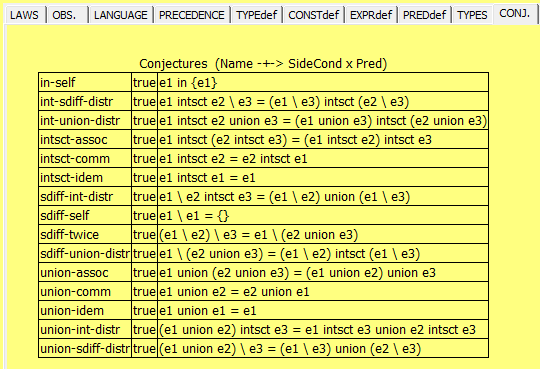
\includegraphics[scale=0.5]{03-set-conjectures.png}

\noindent
Double-clicking on the \texttt{intsct-comm} row (5th) opens up a proof window,
and we use its setup menu to select the ``Reduce'' strategy,
which attempts to transform the goal predicate into TRUE.
Other strategies, depending on the goal structure include: ``left-to-right'',
for equality/equivalence conjectures, that
converts the lefthand side until equal to the righthand side,
or ``reduce-both'' which tries to transform both sides into some common form.

In the proof window we have the goal and side-conditions displayed,
and there is some material about heuristics we ignore in this paper.
The lower half of the proof window displays the ``TARGET'',
determined by the goal and the chosen strategy.
Some context information is also shown, the most important being the free variables,
and the type, in this case, of each side of the equality.
We see the starting goal at the bottom, in bold and underlined%
\footnote{The ``Matches'' subwindow will not be discussed here}%
:

\includegraphics[scale=0.5]{06-starting-REDUCE-proof.png}

\noindent
If we right-click anywhere in the ``Goal and Proof'' subwindow,
then a menu of laws applicable to the goal pops-up.
In effect the goal was matched against all the laws present in the
\texttt{Sets}, \texttt{Equality}, \texttt{Logic} and \texttt{\_ROOT} theories, the successful matches were then ranked
(by various user-selectable heuristics), the top twenty chosen, then applied to the
goal to show the result, and presented in the menu.

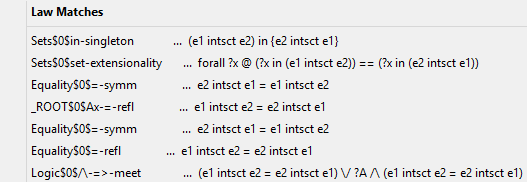
\includegraphics[scale=0.5]{07-laws-applicable-to-goal.png}

\noindent
If we pick the second, ``set-extensionality'', as it has new variables not present in the goal, (e.g. \texttt{?x}), we are asked to supply instances for these, with a reasonable default being offered.
This feature is not obviously useful in this example (except if \texttt{x} was present elsewhere) but comes in handy when matching the rhs of a law like $A \lor (A \land B) \equiv A$, to get the rhs,
in which we are free to instantiate $B$ as we see fit.

  \includegraphics[scale=0.5]{08-instantiating-qvars.png}

\noindent
If we go with the default suggestion, then we obtain the following proof state:

  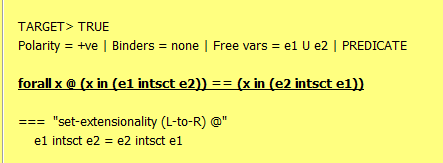
\includegraphics[scale=0.5]{09-extensionality-applied.png}

\noindent
We can use arrow-keys to move around the goal, changing the proof ``focus''.
If we go ``down'' twice, we focus in on the first set membership assertion.
It is worth noting that the line above records that the focus is on an expression (EXPR)
of type boolean (\texttt{B}). \UTP2\ has a on-the-fly type inference algorithm that runs
every time the focus changes%
\footnote{speed has never been a problem with this}%
, and is used by the law matching algorithm to avoid spurious matches.
We avoid lots of explicit type annotations, preferring to deal with such issues
behind the scenes. This is of course in keeping with the general traditional UTP approach
to theorem development.

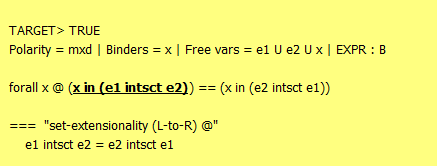
\includegraphics[scale=0.5]{11-moving-down-again.png}

\noindent
Right-clicking now leads to laws relevant to the focus:

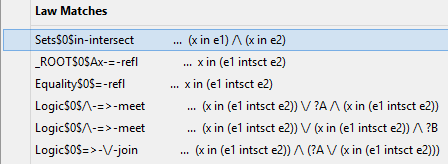
\includegraphics[scale=0.5]{12-laws-applicable-to-focus.png}

\noindent
If we pick the first option, then we get a conjunction of simpler membership statements.

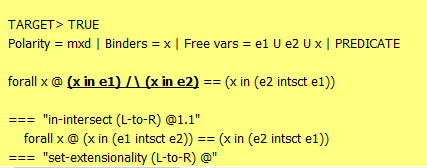
\includegraphics[scale=0.5]{13-intersect-axiom-applied.png}

\noindent
Moving to the righthand side of the equality, we can apply the same \texttt{in-intersect} law,
then apply the commutativity of conjunction, pull back out and we get
instances of the reflexivity of equals. Finally we get rid of a vacuous quantifier,
so resulting in the goal \texttt{TRUE}, and \UTP2\ proclaims!

\includegraphics[scale=0.5]{17-proof-complete.png}

\noindent
Examining the ``THEOREMS'' tab in the Set theory window shows our new theorem.

\includegraphics[scale=0.5]{20-our-new-theorem.png}

\noindent
Right-clicking on it gives another pop-up menu of interesting things to do with it.

  \includegraphics[scale=0.5]{21-saving-text-version.png}

\noindent
We render a simple text version of the resulting proof:
\begin{verbatim}
Complete Proof for 'Sets$intsct-comm
Goal : e1 intsct e2 = e2 intsct e1
Strategy: Reduce to TRUE

     e1 intsct e2 = e2 intsct e1
 ===   " set-extensionality (L-to-R) @ "
     forall x @ (x in (e1 intsct e2)) == (x in (e2 intsct e1))
 ===   " in-intersect (L-to-R) @1.1 "
     forall x @ (x in e1) /\ (x in e2) == (x in (e2 intsct e1))
 ===   " in-intersect (L-to-R) @1.2 "
     forall x @ (x in e1) /\ (x in e2) == (x in e2) /\ (x in e1)
 ===   " /\-comm (R-to-L) @1.2 "
     forall x @ (x in e1) /\ (x in e2) == (x in e1) /\ (x in e2)
 ===   " Ax-==-id (R-to-L) @1 "
     forall x @ TRUE
 ===   " forall-vac (L-to-R) @ "
     TRUE
\end{verbatim}

\noindent
We have only skimmed over the interactive proof features of \UTP2 here.
Others include
\begin{itemize}
  \item keyboard shortcuts to apply built-in procedures to the focus,
    e.g., convert to disjunctive normal form
  \item
    a clickable help feature in the proof window
  \item strategies to support inductive proofs
  \item
    all tables in each tab of each theory can be edited, with entries added
    or deleted --- even laws!
  \item
    Some of the tabs, (``OBS.'',``LANGUAGE'',``PRECEDENCE'') have
    tables that support user definitions of languages.
    See \cite{conf/utp/Butterfield12} for further details.
\end{itemize}


\section{Discussion}

Proofs done with \UTP2 are, in our opinion, more ``open'',
in that we can easily see the steps and laws used in a proof, in an equational style.
A consequence of this is readily seen when we consider the students taking the
Formal Methods course offered at Trinity College Dublin, that focusses on the
UTP, and uses \UTP2 for part of the classwork.
The feedback obtained from these students shows clearly that
(i) the learning curve to get good at \UTP2 proofs is fairly shallow---they almost never
get ``stuck'', once a few tricks are shown---experimentation is easy;
(ii) their concerns are regarding improvement to the GUI itself,
either in terms of how it looks, or having the flexibility to define their own keyboard
shortcuts.
A key feature that reduces the learning curve is the ability
of the prover to suggest possible next steps, by doing advance pattern-matching
and instantiation.

Proofs in CoQ or Isabelle/HOL are, again in this authors words, more ``procedural'',
and ``opaque'', but definitely more powerful. The disadvantage is that the learning
curve is much steeper, particularly when early success it obtained by tactics like
\texttt{auto}, \texttt{simp} or \texttt{sledgehammer}.
When these fail, the best approach is not so clear to the beginner.
However, there is undeniable power once that learning curve has been climbed.

\UTP2 was really developed to assist in the development of new semantic theories
within the UTP framework. Others have also put effort into doing this for UTP
using both ProofPowerZ\cite{conf/utp/ZC08}
and Isabelle/HOL\cite{conf/vstte/FeliachiGW12,conf/utp/FZW14}.
The price they pay is having to recast material in the ProofPower/HL style.
The benefit they tap into is the power of their proof engines.

The key questions raised here are:
\begin{itemize}
  \item Should point-n-click GUIs be added to existing provers?
  \item To what extent are front-ends like Proof-General or jEdit
  are step in this direction?
  \item
    Should more attention be paid to developing equational reasoning approaches?
  \item
  Can the \UTP2 front-end be fruitfully turned into a wrapper around Isabelle/HOL say?
  \item
  Should it use Isabelle/HOL as a way to check its proofs
  (would save trying to develop a small safe LCF-style kernel for \UTP2) ?
  \item
   Can we envisage proofs been done using gestures on a tablet?
\end{itemize}
Very recent work, presented as Tutorial 2 at FM2014 in Singapore, by Jim Woodcock, Simon Foster
and Frank Zeyda of the University of York, showed an encoding of UTP and some key theories
into Isabelle/HOL. One the negative side, they had to employ further nested quotation schemes,
but on the positive side, they used Isar in such a way that it may be relatively easy to use
Isabelle/HOL to check proof steps made by \UTP2. We hope to explore this connection in the near future.

\subsection{Obtaining Code}

\UTP2 is written in Haskell using the wxHaskell GUI library,
and is available open-source, currently under a GPL v2 license,
from \url{https://bitbucket.org/andrewbutterfield/saoithin}.
The screenshots in this paper were produced using version 0.98a.


\bibliographystyle{eptcs}
\bibliography{UITP2014-MAIN}

\appendix

%\newpage
%\section{Proof Walkthrough}\label{sec:walkthrough}

\begin{enumerate}
  \item Initial state
  \\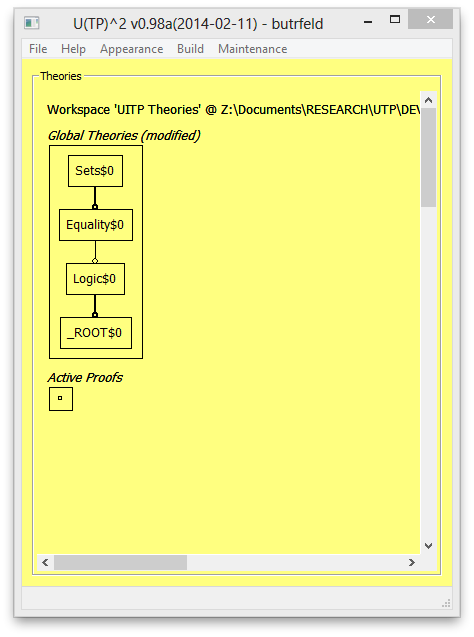
\includegraphics[scale=0.5]{SCREENSHOTS/01-initial-state.png}
  \item Set axioms
  \\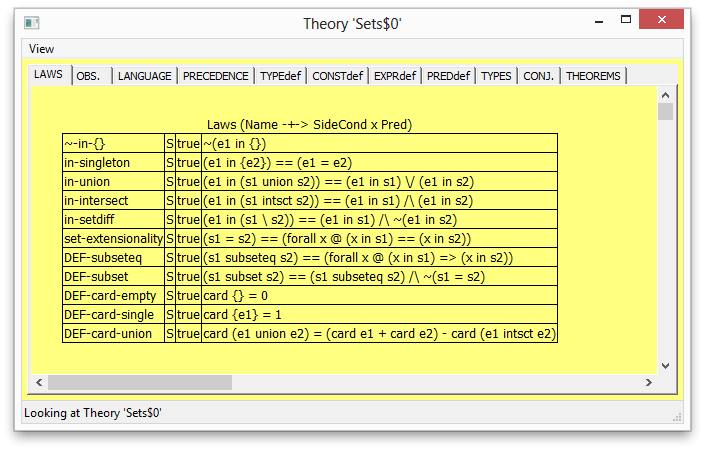
\includegraphics[scale=0.5]{SCREENSHOTS/02-set-axioms.png}
  \newpage
  \item Set Conjectures
  \\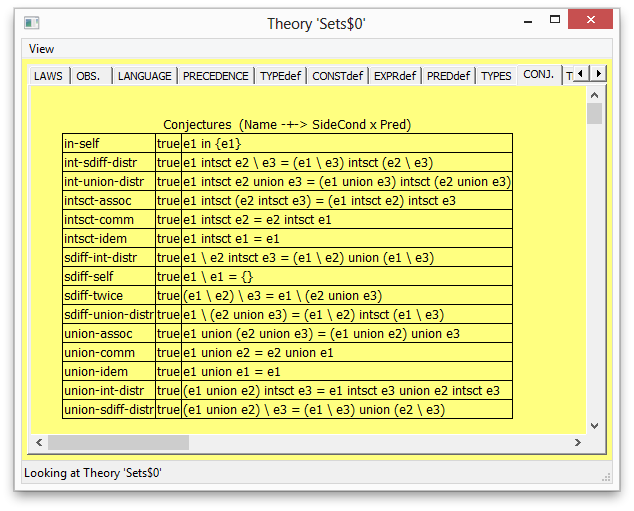
\includegraphics[scale=0.5]{SCREENSHOTS/03-set-conjectures.png}
  \item Starting Proof
  \\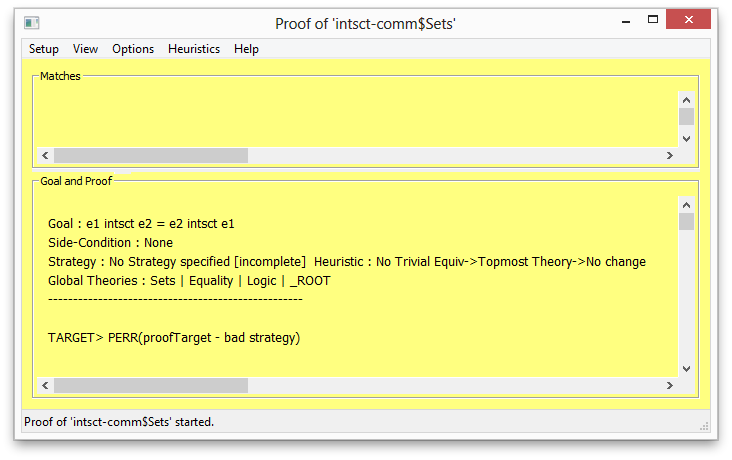
\includegraphics[scale=0.5]{SCREENSHOTS/04-starting-proof.png}
  \newpage
  \item Proof Setup menu
  \\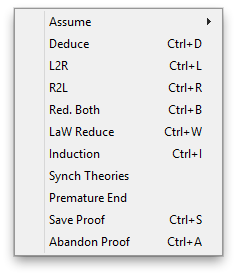
\includegraphics[scale=0.5]{SCREENSHOTS/05-proof-setup-menu.png}
  \item Starting REDUCE Proof
  \\\includegraphics[scale=0.5]{SCREENSHOTS/06-starting-REDUCE-proof.png}
  \newpage
  \item Laws Applicable to top goal
  \\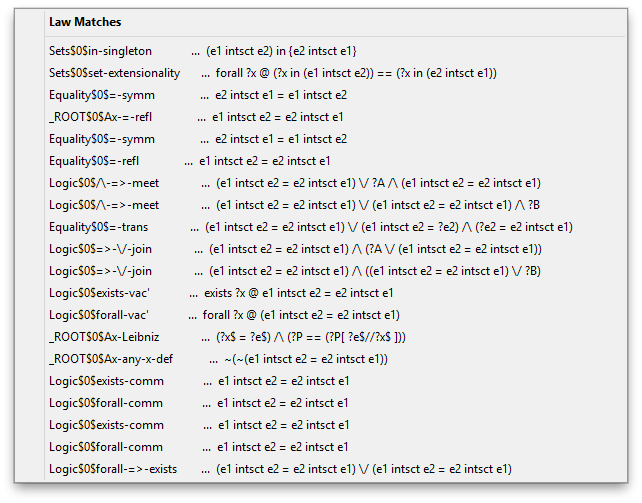
\includegraphics[scale=0.5]{SCREENSHOTS/07-laws-applicable-to-goal.png}
  \item Instantiating Bound Variables
  \\\includegraphics[scale=0.5]{SCREENSHOTS/08-instantiating-qvars.png}
  \newpage
  \item Applying Set Extensionality
  \\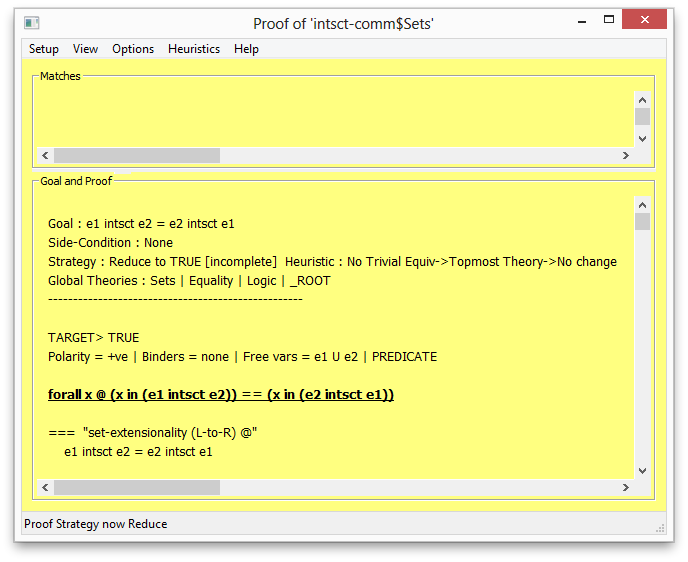
\includegraphics[scale=0.5]{SCREENSHOTS/09-extensionality-applied.png}
  \item Moving Down (down-arrow)
  \\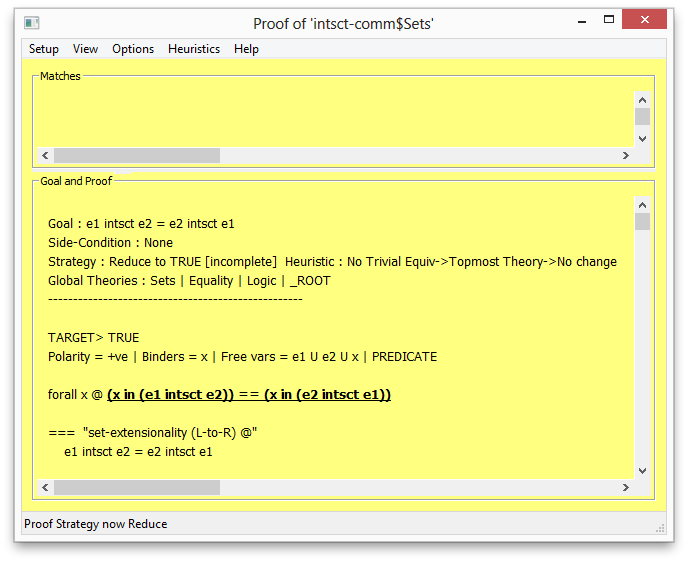
\includegraphics[scale=0.5]{SCREENSHOTS/10-moving-down.png}
  \newpage
  \item Moving Down again (down-arrow)
  \\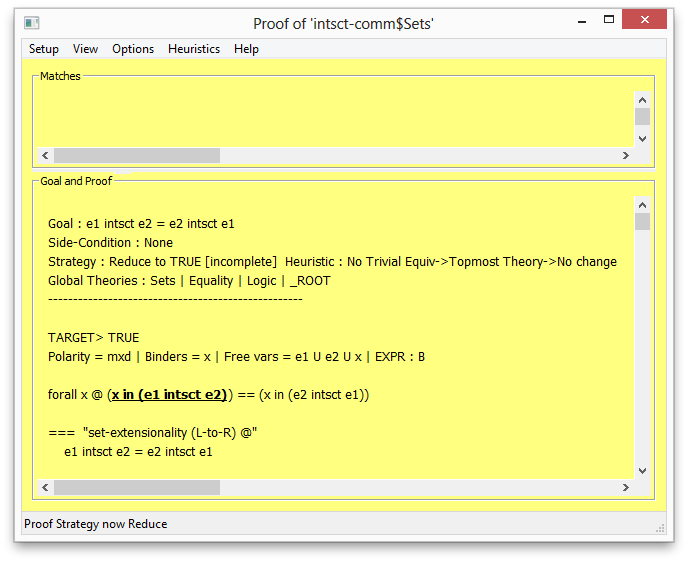
\includegraphics[scale=0.5]{SCREENSHOTS/11-moving-down-again.png}
  \item Laws applicable to current focus
  \\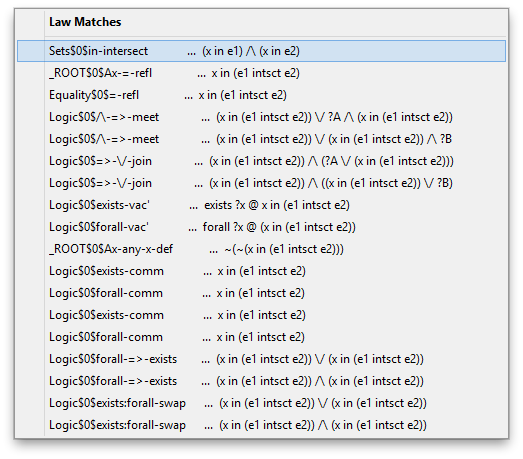
\includegraphics[scale=0.5]{SCREENSHOTS/12-laws-applicable-to-focus.png}
  \newpage
  \item Applying intersection axiom.
  \\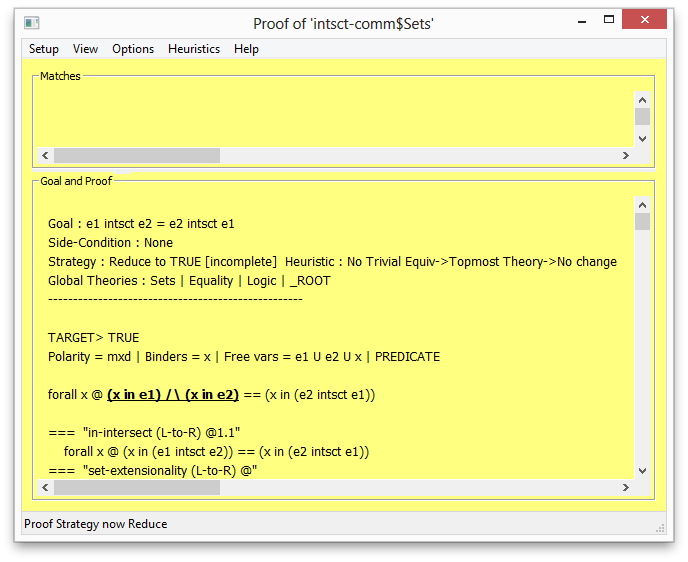
\includegraphics[scale=0.5]{SCREENSHOTS/13-intersect-axiom-applied.png}
  \item Applying commutativity
  \\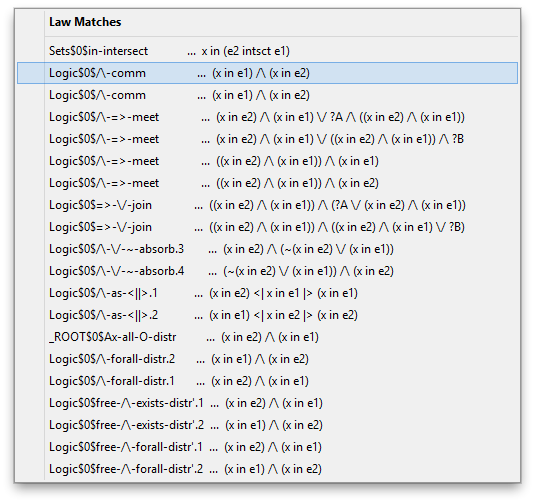
\includegraphics[scale=0.5]{SCREENSHOTS/14-applying-commutativity.png}
  \newpage
  \item Apply Reflexivity of Equality
  \\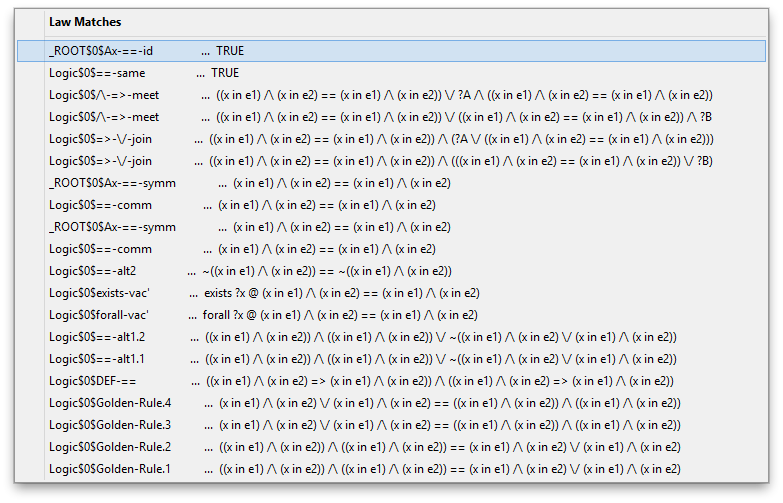
\includegraphics[scale=0.5]{SCREENSHOTS/15-applying-equal-reflexive.png}
  \item Eliminating Vacuous quantifier
  \\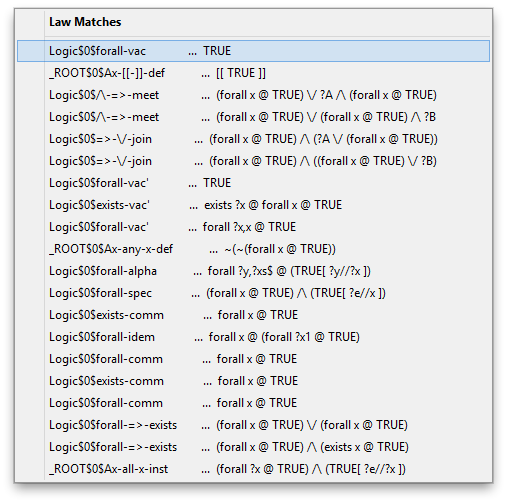
\includegraphics[scale=0.5]{SCREENSHOTS/16-vacuous-quantifier.png}
  \newpage
  \item Proof now complete
  \\\includegraphics[scale=0.5]{SCREENSHOTS/17-proof-complete.png}
  \item Finished Proof
  \\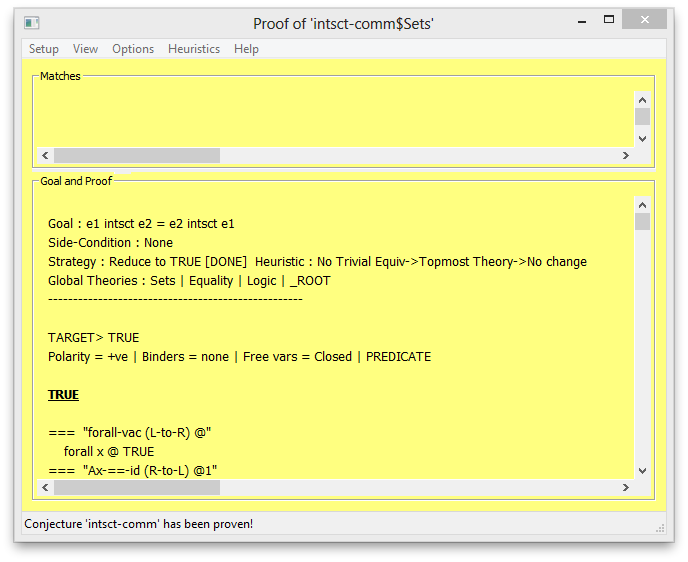
\includegraphics[scale=0.5]{SCREENSHOTS/18-finished-proof.png}
  \newpage
  \item New Theorem added into Law pool.
  \\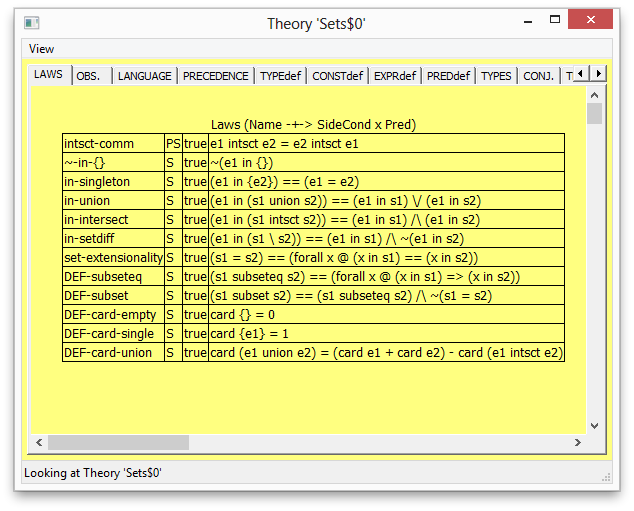
\includegraphics[scale=0.5]{SCREENSHOTS/19-laws-with-new-theorem-added.png}
  \item The new Theorem
  \\\includegraphics[scale=0.5]{SCREENSHOTS/20-our-new-theorem.png}
  \item Saving a Text Version
  \\\includegraphics[scale=0.5]{SCREENSHOTS/21-saving-text-version.png}
  \newpage
  \item Final State
  \\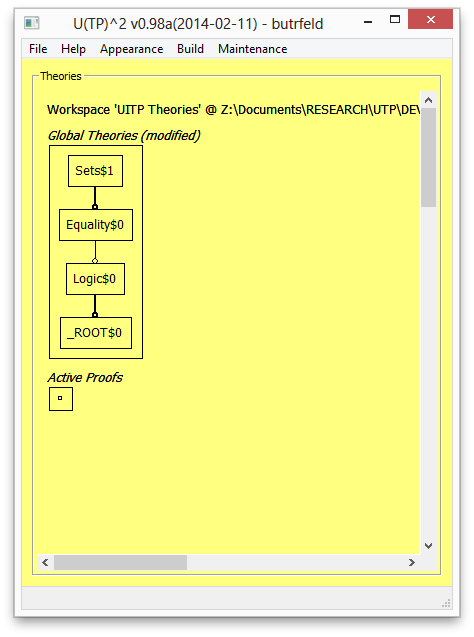
\includegraphics[scale=0.5]{SCREENSHOTS/22-final-state.png}
  \end{enumerate}

The proof text:
\begin{verbatim}
Complete Proof for 'Sets$intsct-comm
Goal : e1 intsct e2 = e2 intsct e1
Strategy: Reduce to TRUE

     e1 intsct e2 = e2 intsct e1
 ===   " set-extensionality (L-to-R) @ "
     forall x @ (x in (e1 intsct e2)) == (x in (e2 intsct e1))
 ===   " in-intersect (L-to-R) @1.1 "
     forall x @ (x in e1) /\ (x in e2) == (x in (e2 intsct e1))
 ===   " in-intersect (L-to-R) @1.2 "
     forall x @ (x in e1) /\ (x in e2) == (x in e2) /\ (x in e1)
 ===   " /\-comm (R-to-L) @1.2 "
     forall x @ (x in e1) /\ (x in e2) == (x in e1) /\ (x in e2)
 ===   " Ax-==-id (R-to-L) @1 "
     forall x @ TRUE
 ===   " forall-vac (L-to-R) @ "
     TRUE
\end{verbatim}


%\newpage
%\section{UTP 2010 Stuff}

\section{Introduction}

\STHN\footnote{Pronounced ``See-heen''.}
is an experimental proof assistant for the logic used in UTP,
supporting a notion of UTP theory, an intuitive prover interface
that supports the equational reasoning style that is prevalent in \cite{UTP-book}
and much other UTP-related literature,
with facilities for the user to define the syntax and semantics
of their own language constructs.
The tool consists of a core equational prover we have developed
in concert with a closely-coupled GUI interface.
At present its focus is on supporting foundational work in developing UTP,
rather than the application of the theory to a ``real-world'' design problem.


\subsection{Motivation}

We are doing foundational work in the UTP \cite{UTP-book},
which requires formal reasoning with not only predicates,
but also predicate transformers: $\RR3(P)$ $\defs$ $\Skip \cond{wait} P$
and predicates over predicates: $P = \RR3(P)$.
We also need to use recursion at the predicate level:
$ P \defs \mu Q \bullet F(Q)$,
as well as partially-defined expressions:
$s \le s \cat (tr'-tr) \equiv  tr \le tr'$.
The logic being used is therefore semi-classical
(two-valued logic, but expressions may be undefined)
and of least 2nd-order.
In addition, tool support for foundational work in UTP requires the ability
to easily describe new language constructs,
which can themselves be treated just like predicates,
in keeping with the ``programs are predicates''
philosophy \cite{conf/mlpl/Hoare85} of UTP.


\subsection{Structure}

We next discuss related work (\S\ref{sec:related}) in order to better justify
our decision to ``grow our own'' theorem proving assistant.
We then proceed to look at the logic (\S\ref{sec:logic:foundation},
type-system (\S\ref{sec:types:foundation}),
user defined language support (\S\ref{sec:language:foundation}),
proof procedures (\S\ref{sec:proof:foundation}),
and law matching (\S\ref{sec:match:foundation},
with emphasis on the underlying foundations.
We then discuss useability and experience (\S\ref{sec:usage})
and finally finish with  future work and conclusions (\S\ref{sec:conclusions}).

\section{Related Work}
\label{sec:related}

There are a lot of theorem provers in existence,
of which the most prominent feature in \cite{conf/tphol/2006provers}.
Of these, the most obvious candidates for consideration for UTP prover support
are Isabelle/HOL\cite{books/sp/NipkowPW02},
PVS\cite{conf/fmcad/Shankar96},
and Coq \cite{bk:Coq'Art:04}.
They are powerful, well-supported,
with decades of development experience
and large active user communities.
They all support higher-order logic of some form, with a command-line interface,
typically based around tactics of some form. All three require functions to be total,
but support some kind of mechanism for handling partial functions
(e.g. dependent types in PVS).
Their reasoning frameworks are based on some form of sequent calculus,
and do not support equational reasoning in a native fashion.

There has been work done on improving the user interfaces
of the above theorem provers.
An interesting example was ``proof by pointing'' \cite{conf/tacs/BertotKT94}
for CoQ which allowed the user to select a subterm,
whereupon it would generate and apply a tactic based on the subterm's top-level
operator.
Whilst proof-by-pointing is not supported in more recent versions of CoQ,
it has been incorporated into ``Proof General'' \cite{conf/tacas/Aspinall00},
a general purpose user interface for theorem provers, built on top of Emacs.
It supports Isabelle and Coq, among others,
and is basically a proof-script management system.
In essence it supports the command-line tactics of the provers,
allowing the user to edit proof scripts at will,
whilst maintaining prover consistency behind the scenes.

Within the UTP community,
there has been considerable work using Proof{\-}Power-Z to
build models of UTP theories in Z in order to mechanise proofs.
Early work looked at deep embedding into Z of an imperative language whose semantics
were given using UTP \cite{conf/utp/NukaW06}.
Work extending this to a mechanisation of UTP itself was also undertaken,
driven by a desire to mechanically verify the semantics of Circus \cite{journals/fac/OliveiraCW09}.
Recent work has looked at re-working the mechanisation of UTP in order to better support
the hierarchical nature of UTP theory building \cite{journals/entcs/ZeydaC09},
where alphabetised predicates are restricted to relations, then designs, and so on.
Some support for Z-like theories from UTP (such as Circus)
can be found as extensions implemented in the Community Z Tools project
\cite{conf/zum/MalikU05}.


Whilst all of good pedigree, CoQ, Isabelle/HOL, ProofPower-Z and PVS
all have in common that they work best when used in the manner
for which they were designed%
---in none of these cases does this manner match the way
we wish to work in UTP, as described in the introduction.
Ironically, the key inspiration for the design of \STHN\ came not from the
above provers, but instead from the one provided as part
of the RAISE Development Method \cite{bk:Raise-dev-mthd:95}.
That theorem prover had mechanisms for selecting sub-expressions
and identifying applicable laws for that sub-expression,
a feature very close to that required for the proof style that \STHN\ supports.


%
%\newpage
%\section{UTP 2012 Stuff}

\section{Introduction}\label{sec:intro}

\PLAN{An introduction to the paper as a rolling case-study.}

Unifying Theories of Programming (UTP) \cite{UTP-book},
is a framework that uses alphabetised predicates to define language
semantics in a relational calculus style, in a way that facilitates
the unification of otherwise disjoint semantic theories,
either by merging them, or using special linking predicates
that form a Galois connection. The framework is designed
to cover the spectrum from abstract specifications
all the way down to near-machine level descriptions,
and as a consequence the notion of refinement plays a key role.

Typically the development of a UTP theory involves determining the
key observational variables, so fixing the alphabet,
then defining healthiness conditions to characterise the predicates
that describe feasible behaviour, introducing the language under study
as a signature, and giving meaning to that signature using healthy predicates.
Algebraic laws of the language can then be developed.

In \cite{conf/utp/Butterfield10}
we gave an overview of the Unifying Theories of Programming Theorem Prover
(\UTP2)
that we are developing to support such theory development work%
\footnote{%
In that paper it was called \STHN, but the name has since changed to \UTP2
}%
.
The prover is an interactive tool, with a graphical user-interface,
designed to make it easy to define a UTP theory and to experiment
and perform the key foundational proofs.
The motivation for developing this tool,
rather than using an existing one has been discussed in some detail
in \cite{conf/utp/Butterfield10}.
We do not repeat it here in the introduction,
but this paper effectively gives a technical underpinning to that motivation.
In this paper we describe the logic behind \UTP2,
starting from 1st-order equational logic \cite{journals/logcom/Tourlakis01},
and gradually exposing the extensions required to facilitate the kind
of reasoning we require for foundational work.
In effect this paper explores the proof infrastructure needed
to reason about a theory of a simple imperative language ($While$),
built upon a theory of ``Designs'',
itself layered on top of a generic UTP base theory.
We start at the bottom looking at the logic and work up until
we can see what is needed for the $While$ language.

This paper assumes that the reader is familiar
with the basic ideas behind UTP, and does not give an introduction
to the subject. A good introduction is the key textbook written
by C.A.R. Hoare and He Jifeng \cite{UTP-book},
which is free to download from \texttt{unifyingtheories.org}.

In the rest of this paper, we use the term ``user'' to
refer to a UTP practitioner  involved in the development
of new UTP theories, and not a software developer
who might want to employ a formal method whose underlying semantics
derive from UTP.

\subsection{Structure of this paper}

Section \ref{sec:theories} talks about theories,
and gives a visual outline of much of this paper
in Figure \ref{fig:hier-of-theory}.
Section \ref{sec:logic} introduces the logic of \UTP2,
and
Section \ref{sec:utp} gives us an introduction to definitions
common to most theories.
In
Section \ref{sec:designs},
and
Section \ref{sec:programs},
we describe how \texttt{Theory}s can be layered up to present
a UTP Theory of Designs, as well as a theory for a simple While programming
language built as an extension on top of Designs.
Section \ref{sec:soundness}
and
Section \ref{sec:exploitation} discuss issues to do with the trustworthiness
and usefulness of \UTP2,
and finally,
Section \ref{sec:conclusions} concludes.
A collection of relevant rules can be found in
Appendix \ref{sec:rules}.


%
%\newpage
%\section{UTP 2014 Stuff}

\section{Introduction}\label{sec:intro}

Unifying Theories of Programming (UTP) \cite{UTP-book},
is a framework that uses alphabetised predicates to define language
semantics in a relational calculus style, in a way that facilitates
the unification of otherwise disjoint semantic theories,
either by merging them, or using special linking predicates
that form a Galois connection. The framework is designed
to cover the spectrum from abstract specifications
all the way down to near-machine level descriptions,
and as a consequence the notion of refinement plays a key role.

In \cite{conf/utp/Butterfield10}
we gave an overview of the Unifying Theories of Programming Theorem Prover
(\UTP2)
that we are developing to support such theory development work%
\footnote{%
In that paper it was called \STHN, but the name has since changed to \UTP2
}%
.
The prover is an interactive tool, with a graphical user-interface,
designed to make it easy to define a UTP theory and to experiment
and perform the key foundational proofs.
The motivation for developing this tool,
rather than using an existing one has been discussed in some detail
in \cite{conf/utp/Butterfield10} and the  technical underpinning has been further elaborated upon in \cite{conf/utp/Butterfield12}.

Here we focus on a small subset of the logic and laws
in order to explain the key role of the extended matcher at the heart of \UTP2.
The focus is on the various matching and inference mechanisms and how they
interact to facilitate the application of laws in a proof at a level
that matches typical handwritten proof steps,
to the extent that this is feasible.

This paper assumes that the reader is familiar
with the basic ideas behind UTP, and does not give an introduction
to the subject. A good introduction is the key textbook written
by C.A.R. Hoare and He Jifeng \cite{UTP-book},
which is free to download from \texttt{unifyingtheories.org}.


\subsection{Matching: an overview}

The matching problem we consider in this paper can be summarised as follows:
during the course of a proof of some conjecture, we will have identified a sub-part
of the proof goal predicate that is of current interest---the \emph{target} focus predicate;
We will then indicate some collection of laws we hope might be applicable,
and then proceed to systematically match the target against those laws,
viewed as \emph{pattern} predicates.
The conjecture will have associated side-conditions,
as will each law---these are added to the match algorithm inputs.
A successful match returns a binding that maps all pattern variables
to the corresponding sub-parts of the target
($\pfun$ is a partial function arrow, while $\ffun$ is a finite partial function).
\[
match : (Pred\times Side) \fun (Pred\times Side) \pfun (Var \ffun \mbox{``Syntax''})
\]
Assuming some success, we can then choose from the range of successful matches,
and use this to apply the law.

In an equational reasoning system such as this, if we match a target
against a law successfully, then it is an instance of such a law,
hence universally true (this is what it means to be a law),
and so the only sensible replacement for the target is the constant predicate \True.
So, why do we return any bindings? Why not just a success/fail indicator?
There are two reasons, one algorithmic and pragmatic,
the other as a result of ensuring maximum flexibility
in the power of the prover:
\begin{enumerate}
  \item a match should fail if different sub-parts of the target
     match different sub-parts of the pattern, but with inconsistent bindings.
     So the attempt to merge these sub-bindings will uncover such problems.
  \item in an equational reasoning system, given law predicates of the
  forms $P \equiv Q$ or $P \implies Q$,
  it makes sense to try matches against either the lhs or rhs,
  with the other side viewed as a template for building the target replacement.
  The binding provides details of how the template should be instantiated.
\end{enumerate}
The process of
finding laws,
establishing if they have the special forms
just described,
 and working out the relevant replacement predicates
($\True$,or one of the law sides),
is fairly straightforward, and we do not discuss it further.

The real focus of this paper is on the function $match$ just introduced
above, and an exposition of how it is so much more than just an exercise
in structural template pattern-matching and merging the resulting bindings.

\subsection{Structure of this paper}

In Section \ref{sec:logic} we introduce a small subset of the logic of \UTP2,
and then in Section \ref{sec:variables} we discuss how the notion
of ``variable'' is neccessarily more complex than in most logic presentations.
In Sections \ref{sec:theories} and \ref{sec:contexts}
we describe how \UTP2 theories provide a context for matching,
while Section \ref{sec:matching} gives an overview of matching,
and Section \ref{sec:struct:matching} describes structural matching,
and its limitations.
The complexities of dealing with those limitation are described in Section \ref{sec:nondet:matching}.
Finally, in Sections \ref{sec:related} and \ref{sec:conclusions} we discuss related work and conclude.


%
%\newpage
%\section{Introduction}

The optional arguments of {\tt $\backslash$documentclass$\{$eptcs$\}$} are
\begin{itemize}
\item at most one of
{\tt adraft},
{\tt submission} or
{\tt preliminary},
\item at most one of {\tt publicdomain} or {\tt copyright},
\item and optionally {\tt creativecommons},
  \begin{itemize}
  \item possibly augmented with
    \begin{itemize}
    \item {\tt noderivs}
    \item or {\tt sharealike},
    \end{itemize}
  \item and possibly augmented with {\tt noncommercial}.
  \end{itemize}
\end{itemize}
We use {\tt adraft} rather than {\tt draft} so as not to confuse hyperref.
The style-file option {\tt submission} is for papers that are
submitted to {\tt $\backslash$event}, where the value of the latter is
to be filled in in line 2 of the tex-file. Use {\tt preliminary} only
for papers that are accepted but not yet published. The final version
of your paper that is to be uploaded at the EPTCS website should have
none of these style-file options.

By means of the style-file option
\href{http://creativecommons.org/about/license/}{creativecommons}
authors equip their paper with a Creative Commons license that allows
everyone to copy, distribute, display, and perform their copyrighted
work and derivative works based upon it, but only if they give credit
the way you request. By invoking the additional style-file option {\tt
noderivs} you let others copy, distribute, display, and perform only
verbatim copies of your work, but not derivative works based upon
it. Alternatively, the {\tt sharealike} option allows others to
distribute derivative works only under a license identical to the
license that governs your work. Finally, you can invoke the option
{\tt noncommercial} that let others copy, distribute, display, and
perform your work and derivative works based upon it for
noncommercial purposes only.

Authors' (multiple) affiliations and emails use the commands
{\tt $\backslash$institute} and {\tt $\backslash$email}.
Both are optional.
Authors should moreover supply
{\tt $\backslash$titlerunning} and {\tt $\backslash$authorrunning},
and in case the copyrightholders are not the authors also
{\tt $\backslash$copyrightholders}.
As illustrated above, heuristic solutions may be called for to share
affiliations. Authors may apply their own creativity here.

Exactly 46 lines fit on a page.
The rest is like any normal {\LaTeX} article.
We will spare you the details.
The rest is like any normal {\LaTeX} article.
We will spare you the details.\\
The rest is like any normal {\LaTeX} article.
We will spare you the details.\\
The rest is like any normal {\LaTeX} article.
We will spare you the details.\\
The rest is like any normal {\LaTeX} article.
We will spare you the details.\\
The rest is like any normal {\LaTeX} article.
We will spare you the details.\hfill6\\
The rest is like any normal {\LaTeX} article.
We will spare you the details.\\
The rest is like any normal {\LaTeX} article.
We will spare you the details.\\
The rest is like any normal {\LaTeX} article.
We will spare you the details.\\
The rest is like any normal {\LaTeX} article.
We will spare you the details.\\
The rest is like any normal {\LaTeX} article.
We will spare you the details.\hfill11\\
The rest is like any normal {\LaTeX} article.
We will spare you the details.\\
The rest is like any normal {\LaTeX} article.
We will spare you the details.

Here starts a new paragraph. The rest is like any normal {\LaTeX} article.
We will spare you the details.
The rest is like any normal {\LaTeX} article.
We will spare you the details.\\
The rest is like any normal {\LaTeX} article.
We will spare you the details.\hfill16\\
The rest is like any normal {\LaTeX} article.
We will spare you the details.\\
The rest is like any normal {\LaTeX} article.
We will spare you the details.\\
The rest is like any normal {\LaTeX} article.
We will spare you the details.\\
The rest is like any normal {\LaTeX} article.
We will spare you the details.\\
The rest is like any normal {\LaTeX} article.
We will spare you the details.\hfill21\\
The rest is like any normal {\LaTeX} article.
We will spare you the details.\\
The rest is like any normal {\LaTeX} article.
We will spare you the details.\\
The rest is like any normal {\LaTeX} article.
We will spare you the details.\\
The rest is like any normal {\LaTeX} article.
We will spare you the details.\\
The rest is like any normal {\LaTeX} article.
We will spare you the details.\hfill26\\
The rest is like any normal {\LaTeX} article.
We will spare you the details.\\
The rest is like any normal {\LaTeX} article.
We will spare you the details.\\
The rest is like any normal {\LaTeX} article.
We will spare you the details.\\
The rest is like any normal {\LaTeX} article.
We will spare you the details.\\
The rest is like any normal {\LaTeX} article.
We will spare you the details.\hfill31\\
The rest is like any normal {\LaTeX} article.
We will spare you the details.\\
The rest is like any normal {\LaTeX} article.
We will spare you the details.\\
The rest is like any normal {\LaTeX} article.
We will spare you the details.\\
The rest is like any normal {\LaTeX} article.
We will spare you the details.\\
The rest is like any normal {\LaTeX} article.
We will spare you the details.\hfill36\\
The rest is like any normal {\LaTeX} article.
We will spare you the details.\\
The rest is like any normal {\LaTeX} article.
We will spare you the details.\\
The rest is like any normal {\LaTeX} article.
We will spare you the details.\\
The rest is like any normal {\LaTeX} article.
We will spare you the details.\\
The rest is like any normal {\LaTeX} article.
We will spare you the details.\hfill41\\
The rest is like any normal {\LaTeX} article.
We will spare you the details.\\
The rest is like any normal {\LaTeX} article.
We will spare you the details.\\
The rest is like any normal {\LaTeX} article.
We will spare you the details.\\
The rest is like any normal {\LaTeX} article.
We will spare you the details.\\
The rest is like any normal {\LaTeX} article.
We will spare you the details.\hfill46\\
The rest is like any normal {\LaTeX} article.
We will spare you the details.
The rest is like any normal {\LaTeX} article.
We will spare you the details.
The rest is like any normal {\LaTeX} article.
We will spare you the details.
The rest is like any normal {\LaTeX} article.
We will spare you the details.
The rest is like any normal {\LaTeX} article.
We will spare you the details.
The rest is like any normal {\LaTeX} article.
We will spare you the details.
The rest is like any normal {\LaTeX} article.
We will spare you the details.
The rest is like any normal {\LaTeX} article.
We will spare you the details.
The rest is like any normal {\LaTeX} article.
We will spare you the details.
The rest is like any normal {\LaTeX} article.
We will spare you the details.
The rest is like any normal {\LaTeX} article.
We will spare you the details.
The rest is like any normal {\LaTeX} article.
We will spare you the details.
The rest is like any normal {\LaTeX} article.
We will spare you the details.
The rest is like any normal {\LaTeX} article.
We will spare you the details.
The rest is like any normal {\LaTeX} article.
We will spare you the details.
The rest is like any normal {\LaTeX} article.
We will spare you the details.
The rest is like any normal {\LaTeX} article.
We will spare you the details.

\section{Prefaces}

Volume editors may create prefaces using this very template,
with {\tt $\backslash$title$\{$Preface$\}$} and {\tt $\backslash$author$\{\}$}.

\section{Bibliography}

We request that you use
\href{http://www.cse.unsw.edu.au/~rvg/EPTCS/eptcs.bst}
{\tt $\backslash$bibliographystyle$\{$eptcs$\}$}
. Compared to the original {\LaTeX}
{\tt $\backslash$biblio\-graphystyle$\{$plain$\}$},
it ignores the field {\tt month}, and uses the extra
bibtex fields {\tt eid}, {\tt doi}, {\tt ee} and {\tt url}.
The first is for electronic identifiers (typically the number $n$
indicating the $n^{\rm th}$ paper in an issue) of papers in electronic
journals that do not use page numbers. The other three are to refer,
with life links, to electronic incarnations of the paper.

Almost all publishers use digital object identifiers (DOIs) as a
persistent way to locate electronic publications. Prefixing the DOI of
any paper with {\tt http://dx.doi.org/} yields a URI that resolves to the
current location (URL) of the response page\footnote{Nowadays, papers
  that are published electronically tend
  to have a \emph{response page} that lists the title, authors and
  abstract of the paper, and links to the actual manifestations of
  the paper (e.g.\ as {\tt dvi}- or {\tt pdf}-file). Sometimes
  publishers charge money to access the paper itself, but the response
  page is always freely available.}
of that paper. When the location of the response page changes (for
instance through a merge of publishers), the DOI of the paper remains
the same and (through an update by the publisher) the corresponding
URI will then resolve to the new location. For that reason a reference
ought to contain the DOI of a paper, with a life link to corresponding
URI, rather than a direct reference or link to the current URL of
publisher's response page. This is the r\^ole of the bibtex field {\tt doi}.
DOIs of papers can often be found through
\url{http://www.crossref.org/guestquery};\footnote{For papers that will appear
  in EPTCS and use \href{http://www.cse.unsw.edu.au/~rvg/EPTCS/eptcs.bst}
  {\tt $\backslash$bibliographystyle$\{$eptcs$\}$} there is no need to
  find DOIs on this website, as EPTCS will look them up for you
  automatically upon submission of a first version of your paper;
  these DOIs can then be incorporated in the final version, together
  with the remaining DOIs that need to found at DBLP or publisher's webpages.}
the second method {\it Search on article title}, only using the {\bf
surname} of the first-listed author, works best.
Other places to find DOIs are DBLP and the response pages for cited
papers (maintained by their publishers).
{\bf EPTCS requires the inclusion of a DOI in each cited paper, when available.}

Often an official publication is only available against payment, but
as a courtesy to readers that do not wish to pay, the authors also
make the paper available free of charge at a repository such as
\url{arXiv.org}. In such a case it is recommended to also refer and
link to the URL of the response page of the paper in such a
repository.  This can be done using the bibtex fields {\tt ee} or {\tt
url}, which are treated as synonyms.  These fields should not be used
to duplicate information that is already provided through the DOI of
the paper.
You can find archival-quality URL's for most recently published papers
in DBLP---they are in the bibtex-field {\tt ee}. In fact, it is often
useful to check your references against DBLP records anyway, or just find
them there in the first place.

When using {\LaTeX} rather than {\tt pdflatex} to typeset your paper, by
default no linebreaking within long URLs is allowed. This leads often
to very ugly output, that moreover is different from the output
generated when using {\tt pdflatex}. This problem is repaired when
invoking \href{http://www.cse.unsw.edu.au/~rvg/EPTCS/breakurl.sty}
{\tt $\backslash$usepackage$\{$breakurl$\}$}: it allows linebreaking
within links and yield the same output as obtained by default with
{\tt pdflatex}.
When invoking {\tt pdflatex}, the package {\tt breakurl} is ignored.


\end{document}
